\chapter{Experimental results \status{new}}
\label{chap:results}
\notyetimplemented{}

\todo[inline]{See the cell population tracking and linear construction with spationtemporal ocntet by Kang et al for a good results section}

	\section{Experimental setup}
	
		data
	
		hardware
		
		software

	\section{Cell detector \status{new}}
		
		Maybe show an example of the MSER detection for each dataset
		
		Say that the parameters for all datasets were equal... means sometime more mser considered than necessary... can be tuned to improve performance at the cost of a bit of manual tunning... can be beneficial for long datasets
		
		\subsection{Performance metrics \statusnew}
			precision, recall, time per image (not multicore)
		
		
		Figure \ref{fig:cell_tracks_detection} displays a temporal view of the detected cells. The vertical axis represents the frame of the sequence. The figure clearly shows that ``cell tracks'' are clearly discernible, even if the number of outliers is significant. For the tracking module it is better to have a higher recall than precision, as outliers can be much more easily discarded than segmented tracks linked.
		\begin{figure}
			  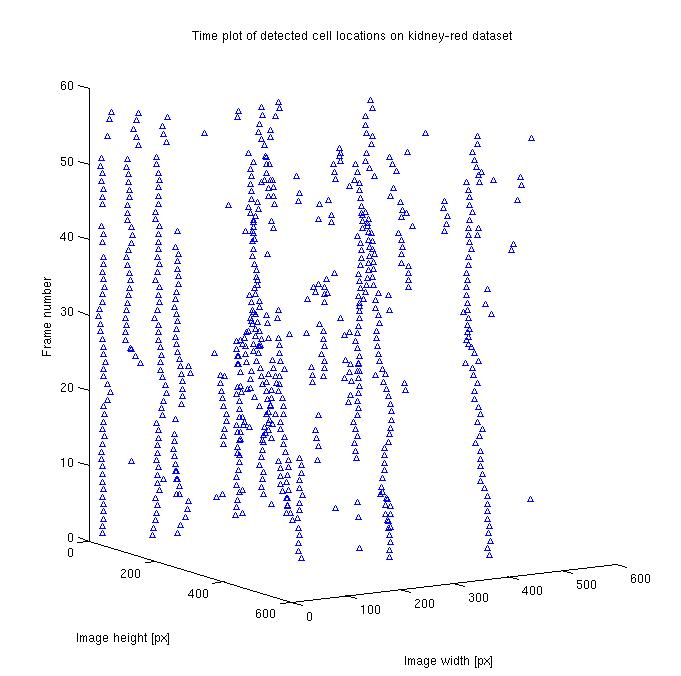
\includegraphics[width=\textwidth]{images/cell_tracks}
			\caption{Cells detected over 60 consecutive frames are visualized as a time series. The vertical axis corresponds to the frames. Even in this raw detection data, it is possible to see the tracks of some of these cells.}
		    \label{fig:cell_tracks_detection}
		\end{figure}
		
		\subsection{Speed \statusnew}
			\todo[inline]{Measure the speed of detection in images of different sizes, and different number of cells}
		
		\subsection{Detection accuracy \statusnew}
			
			- trained on single dataset
			
			- trained on combined dataset
	\section{Cell tracker \statusnew}
		\todo[inline]{Define the different measures of accuracy}
		\subsection{Performance metrics \statusnew}
		
		great Metrics: Research Article, Evaluating Multiple Object Tracking Performance: The CLEAR MOT Metrics
		
		\subsection{Speed \statusnew}
		\todo[inline]{Meause the speed of generating tracks, as a measure of per 1, 100, 1000 frames, depending on the number of tracks}
		\subsection{Tracking accuracy \statusnew}
			- trained on single dataset
						
			- trained on combined dataset
	\section{Limitations and areas of improvement \statusnew}
		Answer: what, why, how to improve in future
		
		- display examples where the tracker did not perform well, and anlyse why. Suggest possible improvement.
		- detection training: only first few frames of datasets, not random -- expect to detect later frames worse
		- testing on only long datasets: no data on short datasets. diffucult to train (what to link?), difficult to annotate
		- speed of detector. Reduce number of hypothesis		

	\section{Summary \statusnew}
	
		Brief review of accuracy... whether it is comparable to other methods in literuature review
		Whether is could be improved in the future... how much